% !TEXroot=main.tex
\section{Navigation}
{	
		Nachdem der Roboter nun auf der durch den Kartenserver bereitgestellten Karte verordnet wurde, muss dem Roboter ein Navigationsziel gegeben werden, damit eine Route zu diesem Punkt berechnet werden kann. Daraufhin soll der Roboter autonom zu diesem Punkt navigieren. Dieser Abschnitt stellt den letzten Schritt des Projekts dar.
		
		\subsection{Navigationsziel festlegen}
		{
			Rviz bietet dazu eine einfache Möglichkeit. In der oberen Leiste kann die Option ``\emph{2D Nav Goal}`` genutzt werden, um graphisch auf der vorliegenden Karte eine Zielposition festzulegen. Diese wird durch einen Pfeil repräsentiert und beinhaltet auch die Blickrichtung (Abbildung \ref{pic:rviznavgoalsmall}).
			\begin{figure}[b]
				\centering
				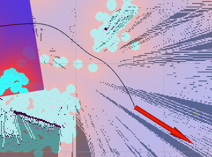
\includegraphics[height=5cm]{Bilder/rviz_navgoal_small.png}
				\caption{Eine in Rviz gesetzte Zielposition} 
				\label{pic:rviznavgoalsmall}
			\end{figure}
		Diese Position wird durch Rviz unter dem \emph{move\textunderscore base\textunderscore simple/goal} - Topic als Nachricht des  \emph{geometry\textunderscore msgs/PoseStamped} - Typs veröffentlicht und damit an die \emph{move\textunderscore base} weitergegeben.
		}
	
		\subsection{Implemention}
		{
			
			
			Die Navigation und Wegplanung geschieht durch das \emph{move\tus base}- Paket. Dabei wird zuerst, wie erwähnt, der grobe Weg, gefolgt von dem exakten Weg im lokalen Bereich berechnet. Dabei wird die durch GMapping erstellte Karte zur Hilfe genommen. Die beigefügte Abbildung  gibt einen Überblick über alle aktiven Nodes. Hierbei stellt das große Rechteck (links) die Komponenten der \emph{move\tus base} dar (Abbildung \ref{pic:rosgfullfront}).
			

			
			Wichtig sind für die Wegplanung hierbei die Parameter der Costmap, da dieser darüber entscheiden, wo der Weg entlang läuft. Dabei spielt das Aufblasen (Inflation) von Hindernissen eine wichtige Rolle. Je stärker ein Objekt aufgeblasen wurde, desto weiter wird es umfahren. Zwar ist ein großer Abstand gut, um Kollisionen zu verhindern, jedoch kann ein Labyrinth nicht viel Platz zwischen den Wänden bieten. Daher können Hindernisse auch nicht so stark aufgeblasen werden. Der Parameter $inflation_radius$ in der Konfigurationsdatei der Costmap beschreibt diesen Wert. Um in dem Labyrinth überhaupt navigieren zu können, ohne dass der Roboter anhält, da er sich im Radius der aufgeblasenen Hindernisse befindet, muss der Wert schon niedrig ($\approx 15\si{cm}$) angesetzt werden. Um das fahren von Kurven zu ermöglichen wurde der Wert auf $10,7 \si{cm}$ gesetzt, was nur $2 \si{mm}$ über dem Roboterradius ist. Dadurch ist der Roboter jedoch in der Lage, in dem Labyrinth weitestgehend problemlos zu navigieren.
			
			Um dem Roboter das befahren von Kurven zu ermöglichen, nutzt man eine funktionalisiert des Turtlebot3-Burger. Dieser kann sich nämlich auf der Stelle drehen. Dadurch muss eine Drehung keinen, vor allem keinen großen Radius haben. Durch das setzten des $min_vel_theta$ Parameters auf $0$, brauch der Roboter für Drehungen nun keine Geschwindigkeit mehr, sondern kann sich im Stand drehen.
			
			\begin{landscape}
				\begin{figure}[htbp]
					\centering
					\fbox{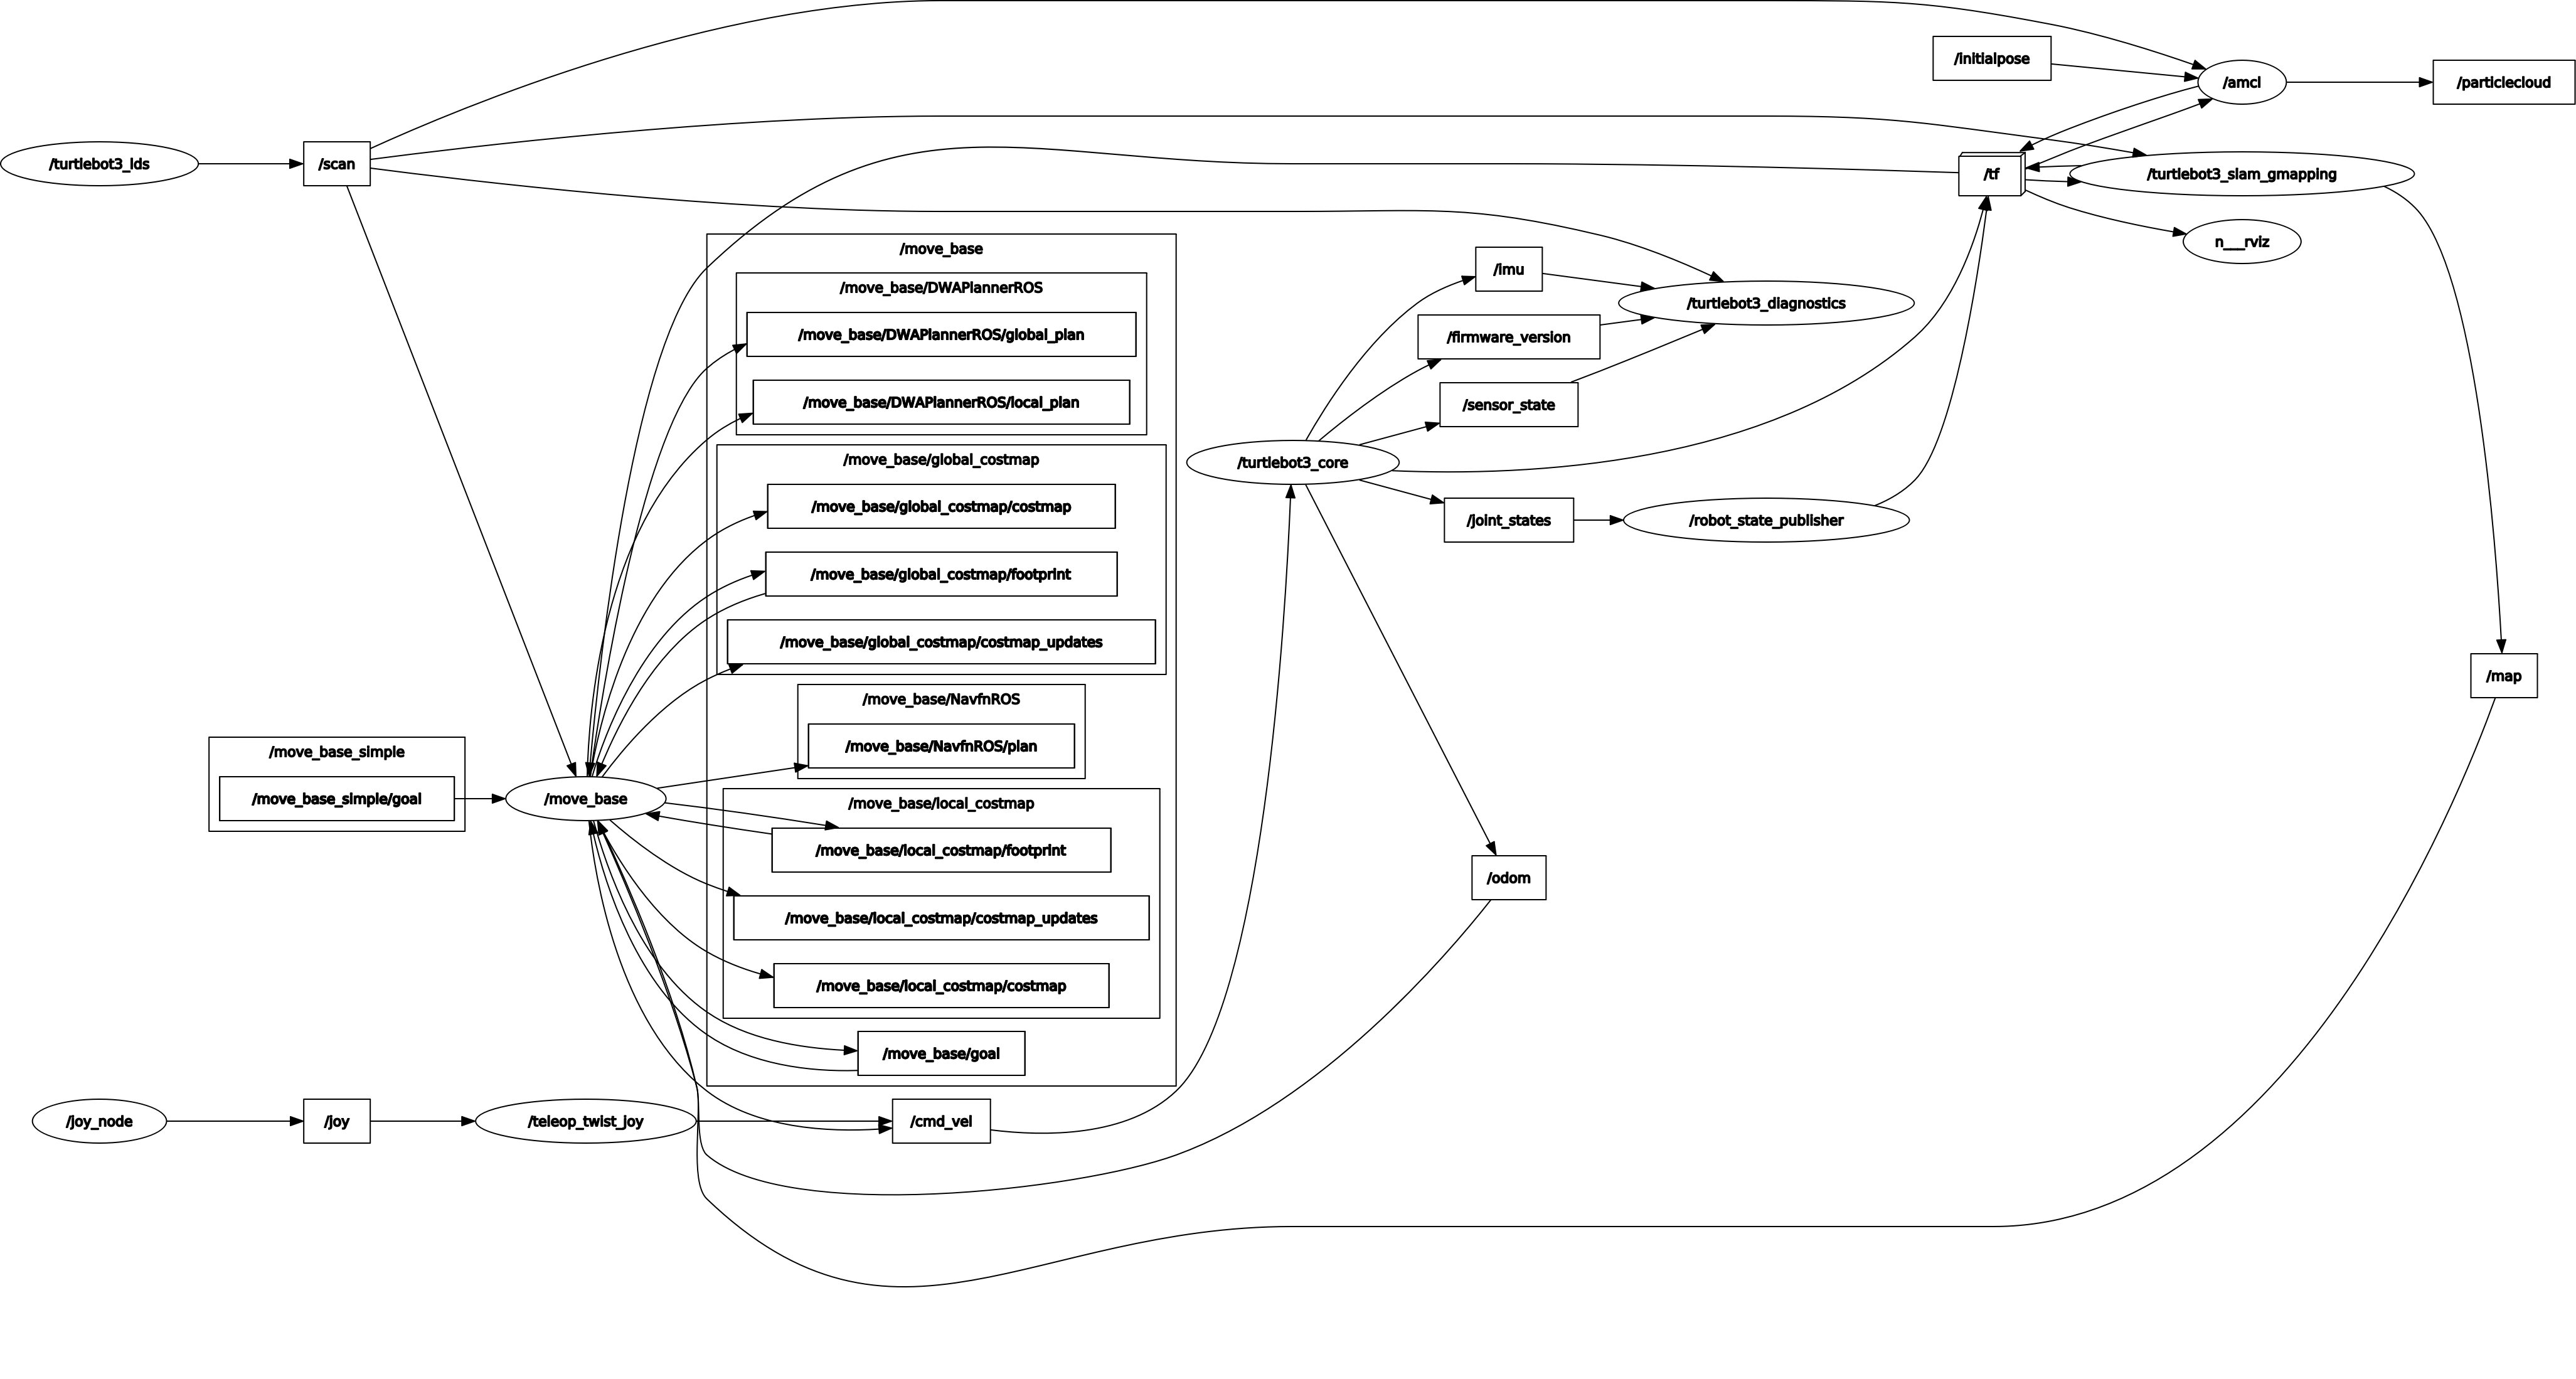
\includegraphics[width=\linewidth, height=\textheight,keepaspectratio]{Bilder/rosgraph_frontier_full.png}} %svg nicht möglich
					\caption[short]{Der gesamte Graph aller aktiven Nodes}
					\label{pic:rosgfullfront}
				\end{figure}
			\end{landscape}

			
			
		}
}	